%--------------第十一章-----------
\chapter{The algebraic $K$-theory spectrum} % (fold)
\label{cha:11the_algebraic_k_theory_spectrum}
In this chapter we apply the ``de-looping machine''(10.4) to the key space $BGLA^+$. We thus have to make a suitable choice for functors $S, T$ and then show that the conditions of (10.4) are satisfied. Choice of $T \colon   \mathbb{R}ing \longrightarrow \mathbb{T}op$\index{Ring@$\mathbb{R}ing$}\index{Top@$\mathbb{T}op$} is obvious: we just compose the general linear group functor $GL \colon   \mathbb{R}ing \longrightarrow \mathbb{G}roup$\index{group@$\mathbb{G}roup$} and the classifying space functor $B \colon   \mathbb{G}roup \longrightarrow \mathbb{T}op$.

$S$ however requires some invention. Various descriptions are available; for our purposes the most convenient is the following, borrowed from Chapter 3. Recall from Chapter 1 that the pseudo-ring $mA$ of finite matrices serves as a copy of $A$ inasmuch as $GLmA \cong GLA$ (1.14). Now $mA$ is a two-sided ideal in the ring $CA$\index{cone of a ring@cone of a ring, $CA$} of locally-finite matrices, entries in $A$ (addition and multiplication as for finite matrices); such matrices have only a finite number of non-zero entries in each row and column. We further insist that the elements of a matrix in $CA$ be drawn from a finite sample of elements of $A$. This extra condition, by ensuring that $CA\cong C\Z \otimes_\Z A$, is invaluable whenever the construction is iterated. (However for present purposes it is quite redundant: it follows from the results below that even when it is omitted the same space $BGLCA^+$ ensues.) In fact $mA$ is the extended ideal $A^e$ under the inclusion $A \hookrightarrow CA$
\[a\mapsto \left(
\begin{array}{c|cc}
 a& 0& \cdots\\
 \hline
0 & \multicolumn{2}{c}{\multirow{2}{*}{$0$}} \\
\vdots&  &\\
\end{array}\right)\]
Therefore define $SA$ to be the quotient ring $CA/mA$. Since the ring homomorphism $Cf \colon   CA_1\longrightarrow CA_2$ induced by a homomorphism $f\colon   A_1 \longrightarrow A_2$ sends $mA_1$ to $mA_2$, the construction $S$ is indeed functorial and serves as this chapter's example for $S \colon   \mathbb{R}ing \longrightarrow \mathbb{R}ing$. Again, for later convenience we note that there is a natural isomorphism between the functors $A \mapsto SA$\index{suspension of a ring, $SA$} and
$A\mapsto S\Z \otimes_\Z A$.

With these choices for $S, T$, the theorem dictated by (10.4) is as follows.
\begin{theorem}
There is a functor from $\mathbb{R}ing$ to the category of $0$-connected $\Omega$-spectra which associates to a ring $A$ the $\Omega$-spectrum $\bar{\mathbf{K}}A$, where $\bar{K}A_{(r)}$ is defined as $(BGLS^rA)_{r+1}^+$ for $r\geqslant 0$ and $\Omega^{-r}(BGLA^+)$ for $r<0$.
\end{theorem}
This result immediately enables us to compare the higlaer $K$-groups of a ring with those of its suspension. By putting $n = 0$ (for example), we obtain that for all $i \geqslant 1$,
\[K_iA = \pi_i(BGLA^+) \cong \pi_i(\Omega(BGLSA)^+_2) = \pi_{i+1}((BGLSA)^+_2).\]
However, after (7.8) this last group is just $\pi_{i+1}(BGLSA^+) =K_{i+1}(SA)$.
\begin{corollary}
  For $i\geqslant  1$, $K_iA\cong K_{i+1}SA$.
\end{corollary}
This is the desired extension of (3.3). Again, it serves to validate the present definition of higher $K$-groups. We may call $\bar{\mathbf{K}}A$ the {\em $0$-connected $K$-theory spectrum}. The corresponding $(-l)$-connected spectrum, $\mathbf{K}A$, is (after (10.5), (3.3) b))
\[KA_{(r)}=
\begin{cases}
  (BGLS^rA)_r^+  \quad r\geqslant  1 ,\\
\Omega^{-r}(K_0A \times BGLA^+)\quad r\leqslant0 .\\
\end{cases}\]
Now (10.6) links the cohomology theories which derive from these spectra. With the notation $\bar{K}A^n(X) = h^n(X; \bar{\mathbf{K}}A) = [X, (BGLS^nA)^+_{n+1} ]$, etc.\ , its output is as follows.
\begin{corollary}
  For a compact CW-complex $X$, the (functorial) sequence
\[\bar{K}A^0(X)\longrightarrow KA^0(X) \longrightarrow H^0(X; K_0A) \longrightarrow \bar{K}A^1 (X)\longrightarrow KA^1 (X) \longrightarrow H^1 (X; K_0A) \longrightarrow \cdots\]
is exact, with the first three terms constituting a split short exact sequence.
\end{corollary}
To return to (11.1) itself, the spaces $(BGLSA)_2$ and $(BGLS^2A)_3$ appearing there have already been identified in a more algebraic way as $BESA$ and $BStS^2 A$ respectively (9.2), a point we pursue below (11.12). The immediate task is to check the requisite hypotheses for (10.4). Specifically we prove in turn $\cdots $

\begin{prop}\label{11.4}
  There is a fibration 
\[BGLA \longrightarrow BGLCA \longrightarrow BESA.\]
 \end{prop} 

\begin{prop}\label{11.5}
  The fibration (\ref{11.4}) is quasi-nilpotent.
 \end{prop} 

\begin{prop}\label{11.6}
  $BGLA^+$ isnilpotent.
 \end{prop} 

\begin{prop}
  $BGLCA$ is acyclic.
 \end{prop} 
The proof of (\ref{11.4}) is very quick. We just take the exact sequences of groups
\[1\longrightarrow GLmA \longrightarrow GLCA \longrightarrow GLSA, \quad ECA\longrightarrow ESA\longrightarrow 1\]
which result from the definition of $SA$, borrow the facts that $GLmA \cong GLA$ and (from (11.7))
that $ECA=GLCA$, and apply the classifying space functor.

For (\ref{11.5}) and (\ref{11.6}) we need to recall, as we did for (3.11), a key fact from group homology theory: an inner automorphism of a group induces the identity automorphism on its homology. Now homology preserves direct limits, and any group is the direct limit of its finitely generated subgroups. So a group automorphism which acts on each finitely generated subgroup as an inner automorphism of that subgroup again acts trivially on the group's homology. Thus to prove that one group acts trivially on the homology of another it suffices to find, for each finite subset of the latter, an inner automorphism of the latter to which the restricted action corresponds. Perhaps the simplest, feasible guarantee of success is the hypothesis of the following lemma (wherein $C_G(H)$ denotes the centralizer in $G$ of a subgroup $H$).
\begin{lemma}
  Suppose $\varinjlim N_\alpha = N \unlhd G$ where, for all $\alpha$, $N_\alpha \leqslant G$ and
  \[G=N.C_G(N_\alpha)\]
Then $G$ (and thereby $G/N$) acts trivially on $H_*(N)$.
\end{lemma}
\begin{proof}
  An arbitrary finite subset of $N$ is contained in some $N_\alpha$. For this $\alpha$ a given element $g \in G$ may be written as
\[g = g_1g_2 \quad g_1\in N, g_2\in C_G(N_\alpha).\]
Then for all $ h \in N_\alpha$
\[ghg^{-1} = g_1(g_2hg_2^{-1})g_1^{-1} = g_1hg_1^{-1}.\]
\end{proof}
It is amusing to note that the particular case where $G$ can be written in the form $G = N_\alpha C_G(N_\alpha )$, which occurs in the proof of (11.5) for example, may also be deduced from (3.11). One attraction of the hypothesis of (11.8) is its iterative potential $\cdots $
\begin{corollary}
  Suppose $\varinjlim = K_\beta =K \unlhd \varinjlim N_\alpha= N \unlhd G$ where, for all $\alpha,\beta$, there holds $N_\alpha \leqslant G, K_\beta \leqslant N$ and
  \[G = N. C_G(N_\alpha ) \mbox{ and } N = K.C_N(K_\beta).\]
Then $G$ acts trivially on $H_*(K)$.
\end{corollary}
For completeness we should also include the corresponding quasi-nilpotence result. Let $\Gamma_G^i N$ be the lower central series of a normal subgroup $N$ ($\Gamma_G^0 N = N$, $\Gamma_G^{i+1}N = [G, \Gamma_G^iN]$). The definition that $G$ act nilpotently on $N$ reduces to $\Gamma_G^k= 1$ for some $k$, or, equivalently, to $N \leqslant \zeta_k(G)$ for the same $k$ ($\zeta_k(G)$ as in (1.6) -- see p. \pageref{page37}).

\begin{prop}
  Suppose $N\unlhd G$ and for some $k$ $\Gamma_G^k N = \varinjlim H_\alpha$ where, for all $\alpha$, $H_\alpha\leqslant G$ and
\[G = \Gamma_G^k N . C_G(H_\alpha).\]
Then $G$ acts nilpotently on $H_*(N)$.
\end{prop}

The proof applies [22 Theorem 2.4] to the $G$-action on the quasi-nilpotent (after (11.8)) fibration
\[B\Gamma_G^k N\longrightarrow BN \longrightarrow B(N/\Gamma_G^k N).\]
(By definition, $G$ acts nilpotently on $N/\Gamma_G^k N$, and hence on its homology.) lt's not necessary to spell out the proof because in the cases of interest to us $N$ is perfect so that always $\Gamma_G^i N = N$ and (11.8) already applies.

Returning then to these relevant cases, we prove (11.5) by showing (11.8) applies to
$N = GLmA = \varinjlim GLM_nA$, $G = GLCA$. Of course it suffices to consider only generators of $G$; thanks to the by-product $GLCA= ECA$ of (11.7) these are elementary matrices of the form $e_{rs}^\gamma$ where $\gamma \in CA$. Now, for each $n$ there is a decomposition ($\mathrm{Ann}$ = annihilator ideal)\index{annihilator ideal@annihilator ideal, $\mathrm{Ann}$}
\[\gamma= \gamma_1+ \gamma_2 \in M_nA + \mathrm{Ann}(M_nA),\]
or equally
\[e_{rs}^{\gamma} = e_{rs}^{\gamma_1}e_{rs}^{\gamma_2}\in GLM_nA.C_{GLCA}(GLM_nA). \]
Likewise, for the action of $GLA$ on $H_*(EA)$, let $g \in GLA$ and $n$ be given. Write $h = \max (n, k)$ where $g \in GL_kA$, and thus 

\[g=\begin{pmatrix}
  \alpha & 0\\
  0 & I\\
\end{pmatrix}\]
with $\alpha \in M_h A$. Now (from (1.9))
\begin{align*}
  g &=\begin{pmatrix}
  \alpha & 0 & \\
  0 &\alpha^{-1} & 0\\
  0 &0& I\\
\end{pmatrix}\begin{pmatrix}
  I_h& 0 & \\
  0 &\alpha & 0\\
  0 &0& I\\
\end{pmatrix} \\
& \in E_{2h}A.C_{GLA}(GL_hA)\\
&  \leqslant EA.C_{GLA}(E_nA).
\end{align*}
The action on homology is thus trivial, making the fibration 
$$BEA \longrightarrow BGLA \longrightarrow K(GLA/EA, 1)$$
quasi-nilpotent. Since $GLA/EA = GLA/PGLA =GLA_{ab}$ (1.11) is certainly a nilpotent group,
(10.3) reveals $BGLA^+$ to be a nilpotent space, verifying (11.6).

This leaves the key result, (11.7), which we prove by showing $GLCA$ conforms to the following model for acyclic (= homologically trivial) groups.\index{acyclic group}
\begin{lemma}
  Suppose a group $G$ is the direct limit of subgroups $G_\lambda$, $\lambda \in \Lambda$, each equipped with a homomorphism $\phi_\lambda\colon   G_\lambda \longrightarrow  C_{G_\mu}(G_\lambda)$, $\lambda \leqslant \mu = \mu_\lambda \in \Lambda$, and an element $a \in G_\mu$ such that for all $g\in G_\lambda$, $g=[a, \phi_\lambda(g)]$. Then $G$ is acyclic.
\end{lemma}
The above lemma is an immediate corollary of (3.11), obtained by letting $\rho \colon   G\longrightarrow G$ be the trivial endomorphism.

To complete the proof of (11.7), and thereby (11.1), we must show that $GLCA = \varinjlim GL_nCA$ fits the framework of this lemma. Crucial here is the existence of a bijection, say $\gamma \colon   \N \longrightarrow  \N \times \N$.
For this induces an isomorphism $\gamma^* \colon   A^{\N\times \N} \longrightarrow  A^\N$ which may be regarded as a re-indexing of bases; thus our original ring $CA$ defined on the countably generated free module $A^\N$ is isomorphic to the ring $\hat{C}A$ of matrices which are locally finite with respect to the module $A^{\N \times \N}$ via $CA \longrightarrow \hat{C}A$, $\alpha \mapsto \gamma^{*-1}\circ \alpha \circ \gamma^* =\hat{\alpha}$. There is then defined a homomorphism
\begin{align*}
\psi \colon  & \hat{C}A \longrightarrow \hat{C}A \\
   & \hat{\alpha} \mapsto [\alpha \oplus  \alpha \oplus \alpha \oplus \cdots\colon   \bigoplus_\N A^\N \longrightarrow \bigoplus_\N A^\N ].
\end{align*}
It is in fact $\psi_* \colon   GL_n(\hat{C}A) \longrightarrow  GL_n(\hat{C}A)$ which we use, to define
\begin{align*}
  \phi_n\colon  & GL_n(\hat{C}A)\longrightarrow GL_{3n}(\hat{C}A) \\
  & \hat{\alpha} \mapsto \begin{pmatrix}
    I_n & 0 & 0\\
    0 & \psi_*\hat{\alpha} & 0\\
    0 & 0& I_n
  \end{pmatrix}
\end{align*}
Evidently $[GL_n(\hat{C}A), \phi GL_n(\hat{C}A)] = 1$, so that it remains to identify a matrix $\mu_n \in GL_{3n}(\hat{C}A)$ with the property that $\hat{\alpha} = [\mu_n, \phi_n(\hat{\alpha})]$. Since it is actually a permutation matrix which does the
trick, the easiest way to describe it is as a permutation of the basis elements, which we write as
$\sideset{^h}{_l}{\mathop{(\sideset{_i}{^k}{\mathop{e}})}} =\sideset{^h_i}{_l}{\mathop{(e^k)}} =\sideset{^h_i}{^k_l}{\mathop{e}} \in \bigoplus_{h=1}^3 \bigoplus_{i=1}^n \bigoplus_{l\in \N} A^\N $.
Just to check this notation, observe that $\phi_n(\hat{\alpha})$ above behaves as
\[\sideset{^h_i}{^k_l}{\mathop{e}} \mapsto \begin{cases}
\sideset{^1_i}{^k_l}{\mathop{e}}    \quad h=1 , \\
\sideset{^2}{_l}{\mathop{(\alpha({\sideset{_1}{^k}{\mathop{e}}}))}}    \quad h= 2, \\
\sideset{^3_i}{^k_l}{\mathop{e}}    \quad h=3 . \\
\end{cases}\]
Now define $\mu_n$ by
\[\sideset{^h_i}{^k_l}{\mathop{e}} \quad \begin{cases}
\sideset{^3_i}{_1}{\mathop{(\gamma^*e_l^k)}}    \quad h=1 , \\
\sideset{^1_i}{}{\mathop{(\gamma^{*-1}e^k)}}    \quad h= 2,l=1, \\
\sideset{^2_i}{^k_{l-1}}{\mathop{e}}    \quad h= 2,l>1, \\
\sideset{^3_i}{^k_{l+1}}{\mathop{e}}    \quad h=3 . \\
\end{cases}\]
The picture of $\mu$ (for each $i$) is rather pretty:
\begin{center}
  \begin{tikzpicture}
  \foreach \x in {1,2,3,4,6,7,8,9,12,13,14,15}
   \foreach \y in {1,2,3,4}
   {
   \draw (\x,\y) circle [radius=0.05];
   }
   \draw [rounded corners] (0.8,0.8) rectangle (4.2,4.2) ;
   \foreach \x in {5.8,6.8,7.8,8.8,11.8,12.8,13.8,14.8}
   {
   \draw [rounded corners] (\x , 0.8) rectangle (\x+0.4,4.2) ;
   }
   \node [left] at (0.8,4) {$k\uparrow$};
   \node [below] at (2.5,0.7) {$h=1$};
   \node [below] at (4,0.8) {$l\rightarrow$};
   \node [below] at (7.5,0.7) {$h=2$};
   \node [below] at (9,0.8) {$l\rightarrow$};
   \node [below] at (13.5,0.7) {$h=3$};
   \node [below] at (15,0.8) {$l\rightarrow$};
   \draw [->] (4.3,0.7) to [out=-45,in=180](8,-.5) to[out=0,in=180] (11.8,2);
   \node [below] at (7,0) {$\gamma^*$};
   \node [right] at (12.2,2) {$\rightarrow$};
   \node [right] at (13.2,2) {$\rightarrow$};
   \node [right] at (14.2,2) {$\rightarrow$};
   \node [right] at (15.2,2) {$\rightarrow$};
    \node [right] at (6.2,3.2) {$\leftarrow$};
    \node [right] at (7.2,3.2) {$\leftarrow$};
    \node [right] at (8.2,3.2) {$\leftarrow$};
    \node [right] at (9.2,3.2) {$\leftarrow$};
    \node [left] at (5.5,3.4) {$\overset{\gamma^{*-1}}{\longleftarrow}$};
\end{tikzpicture}
\end{center}
It is (genuinely) easy to verify that these two matrices have commutator $\hat{\alpha}$ after all. So we are done.

There is a bonus, inasmuch as both $\mu_n$ is always a permutation matrix and $\phi_n(\hat{\alpha})$ is, so long as $\hat{\alpha}$ was. Thus the lemma also establishes the acyclicity of the group of infinite permutations of $\N \times \N$ which leave all but finitely many columns (copies of $\N$) invariant. In fact the lemma serves to establish the acyclicity of many other groups besides, but that, as they say, is another story $\cdots $

Finally, if an infinite delooping of $BGLA^+$ seems like a concept without much algebraic motivation, I can offer the following interpretation of the second stage. The first, you will recall came from the short exact sequence
\[GLA \rightarrowtail GLCA = ECA\twoheadrightarrow ESA .\]
Had we applied (10 1) instead of the more ambitious (10.4), we'd have come across a fibration $BEA \longrightarrow BGLCA \longrightarrow  BStA$ (since $BStA = (BGLA)_3$ (9.2)). Historically, I only suspected that something like (10.1) might hold simply because I had first established the purely algebraic result $\cdots $

\begin{prop}
  There is a short exact sequence
\[EA \rightarrowtail ECA = StCA \twoheadrightarrow StSA .\]
 \end{prop} 
Since a ring epimorphism must induce an epimorphism of Steinberg groups, the proof consists in identifying $K = \ker [StCA \longrightarrow StSA]$. As a first step, note that
\[K \leqslant \ker [ECA = StCA\longrightarrow StSA\longrightarrow ESA] = GLA.\]
To obtain a lower bound for $K$ we argue in the converse direction: because $EA \leqslant GLA$ the homomorphism $EA\longrightarrow  ECA\longrightarrow StSA \longrightarrow ESA$ is trivial, so that $EA\longrightarrow  StSA$ must factor through $\ker [StSA \longrightarrow ESA] = H_2(ESA)$. Actually, we only need the fact that this kernel is abelian as this implies the triviality of the image of any perfect group, such as $EA$. Thus the original homomorphism $EA \longrightarrow StSA$ is also trivial, leaving
\[EA\leqslant K\leqslant GLA .\]

The proof is completed by two-fold application of the exact sequence 
\[H_2(G) \longrightarrow H_2(Q) \longrightarrow  N/[G, N] \longrightarrow G_{ab} \longrightarrow Q_{ab}\]
arising classically from a short exact sequence $N \hookrightarrow G\twoheadrightarrow Q$. In the first instance, from $K \hookrightarrow  ECA\twoheadrightarrow StSA$ we deduce, because $ECA$ is perfect while $StSA$ is superperfect, that $K = [ECA, K]$. In the second, from $GLA \hookrightarrow ECA\twoheadrightarrow ESA$ we have, $ECA$ being superperfect, that
\begin{align*}
 GLA/[ECA,GLA] & \cong H_2(ESA)\\
 &=K_2(SA) \quad \mbox{(by (9.2))} \\
 &=K_1(A) \quad \mbox{(by (3.3)c))} \\
 &=GLA/EA.
\end{align*}
Since $EA= [GLA, GLA] \leqslant [ECA, GLA]$ , it must be that 
\[EA = [ECA, GLA] .\]
This combines with the previous pieces of information to reveal that 
\[EA\leqslant K = [ECA,K] \leqslant [ECA, GLA] = EA,\]
 and hence $K = EA$ after all.
 % chapter the_algebraic_k_theory_spectrum (end)